\documentclass[paper=a4, fontsize=12pt]{scrartcl}
\usepackage[left=32mm,top=25mm,right=32mm,bottom=25mm]{geometry}
\usepackage{titling}
\usepackage{mathtools}
\usepackage{amsmath}

\renewcommand{\thesubsection}{\thesection.\alph{subsection}}
\setlength{\droptitle}{-9em}
\title{\textbf{Algoritmica grafurilor - Tema 2}}
\author{Bucătaru Andreea A2 \and Bulboacă Maria A2}
\date{\normalsize\ 23 noiembrie 2018}

\begin{document}

\maketitle

\section*{Problema 1}
\paragraph{}
$G = (V, E)$ graf conex cu un cuplaj perfect.

Teorema König: Fie $G$ un graf bipartit. Atunci cardinalul maxim al unui cuplaj din $G$ este egal cu cardinalul minim al unei acoperiri cu noduri 
a lui $G$, $\mathit{v}(G) = n - \alpha(G)$.

O formă echivalentă a teoremei lui König: cadinalul mulțimii maxime de puncte independente + cardinalul maxim al cuplajului = numărul de noduri.

(Teorema Norman-Rabin) În orice graf fără noduri izolate (graf conex), cardinalul minim al unei acoperiri cu muchii + cardinalul maxim al cuplajului = 
numărul de noduri. Dacă $\exists$ un cuplaj perfect, atunci cardinalul cuplajului și cardinalul acoperirii cu muchii sunt $|V| \backslash 2$.

Combinând această egalitate cu teorema lui König $\Rightarrow$ în grafuri bipartite, cardinalul minim al unei acoperiri cu muchii = cardinalul mulțimii
maxime de puncte independente, și cardinalul minim al unei acoperiri cu muchii + cardinalul minim al unei acoperiri cu noduri = numărul de noduri.

În grafuri bipartite, cuplajul maxim este egal cu acoperirea minimă cu noduri. Din acest rezultate deducem că acoperirea minimă cu noduri și mulțimea maximă
de puncte independente se pot rezolva în timp polinomial în grafuri bipartite.

Cuplaj perfect $\Rightarrow$ toate nodurile sunt saturate.

Fie M $\in \mathcal{M}_G$ un cuplaj. Un nod $v$ este saturat de către M dacă $d_M(v) = 1$.

Un graf care are un cuplaj perfect are în orice componentă conexă un număr par de noduri.

Dacă $M$ este cuplaj și $P$ este drum alternat relativ la $M$, atunci dintre $\forall$ două muchii consecutive ale lui $P$, exact una aparține lui $M$
(muchiile aparțin alternativ lui $M$ și $E \backslash M$).

Parcurgem sistematic graful $G = (V$$=$$(S,T), E)$ într-o manieră BFS. Pornind de la una din clase, de exemplu $S$, se consideră mulțimea extremităților
drumurilor de creștere posibile, $S \cap E(M)$, și din fiecare astfel de vârf se începe construcția, în paralel, de drumuri alternate. Prima depistare a unui
drum de creștere oprește construcția, oferind lungimea minimă a unui drum de creștere. Complexitatea timp $O(m+n)$ rezultă prin utilizarea listelor de adiacență.

\section*{Problema 2}
\paragraph{}
Trebuie să arătăm că un graf $G$ conține un cuplaj de cardinal $p \Leftrightarrow q(G-S) \leq |S| + |G| - 2p, \forall S \subseteq V(G)$ și $q(G-S)$ este numărul componentelor 
conexe impare ale lui $G$.

Extindem cuplajul de cardinal $p$, adăugând niște noduri și niște muchii.

Teorema Tutte: Un graf $G$ admite cuplaj perfect $\Leftrightarrow q(G-S) \leq |S|, \forall S \subseteq V(G)$.

Demonstrăm $|G| = \frac{1}{2} \ast (V(G) - \underset{X \subseteq V(G)}{max} (q(G-X) - |X|)$.

Adăugăm r noduri și muchii.

$|G| = \frac{1}{2} \ast (V(G) - r_0)$, unde $r_0$ este cel mai mic $r$ astfel încât $G_r$ are un cuplaj perfect.

Folosim teorema Tutte pentru a identifica acele $G_r$ care au cuplaje perfecte și a afla $r_0$.

   
\section*{Problema 3}
\paragraph{a)}
Fie arborele parțial de cost minim H, construit pe baza lui G. Conform teoremei generale MST, H poate fi format din doi arbori parțiali
(fie ei $Hs, Ht$) de cost minim pentru oricare două submulțimi de vârfuri disjuncte $S,T \in V(G)$ unite printr-o muchie de cost minim $e=(u,v)$
astfel încât $u \in S$ și $v \in T$. Deci $e \in E(H)$. Există un $Hs$ și un $Ht$ pentru orice muchie $e \in E(H)$.

Fie tăietura $A \in E(G)$ care să realizeze o bipartiție $(S,T)$ astfel încât $G-A$ să fie neconex și $e \in A$. Presupunem prin reducere
la absurd că $e$ nu e de cost minim în această tăietură: $c(e) \neq \underset{x \in A}{min}$ $c(x)$.

Avem MST-urile $Hs$ și $Ht$ și dorim să îl creăm pe $H$. Alegem muchia $e'$ astfel încât $c(e') = \underset{x \in A}{min}$ $c(x)$. Dar dacă
$c(e') < c(e)$ înseamnă că $H$ nu este MST, ceea ce este o contradicție pentru ipoteza inițială. Deci, $e$ este de cost minim în tăietura $A$.

Astfel, orice muchie $e \in E(H)$ trebuie să fie de cost minim într-o tăietură.

\paragraph{b)}
Fie un circuit $C$ și o muchie $e \in E(C)$, cu $c(e) = \underset{x \in E(C)}{max}$$c(x)$. $C$ conține muchiile: $(u_1, u_2), (u_2, u_3), ..., (u_{i-1}, u_i), (u_i, u_{i+1}), ..., (u_n, u_1)$.
Fie muchia $e = (u_{i-1}, u_i)$.

Considerăm arborele parțial de cost minim $H$, format pentru subgraful cu vârfurile: $V_H = \{u_1, ..., u_{i-2}, u_{i+1}, ..., u_n\}$.
Extindem acest arbore parțial de cost minim pentru a-l conține și pe $u_{i-1}$ printr-o muchie oarecare $e'$ (din subgraful cu $V = V_H$).
Presupunem prin reducere la absurd că pentru a-l include apoi în noul arbore $H$ și pe $u_i$, alegem muchia $e$ de cost maxim.
Dar, cum $H$ îl conține și pe $u_{i+1}$ și avem muchia $(u_i, u_{i+1})$, iar $c((u_i, u_{i+1})) < c(e)$, arborele rezultat nu ar mai fi de cost minim 
(deoarece am ales o muchie mai costisitoare) $\Rightarrow$ contradicție $\Rightarrow e$ nu poate face parte dintr-un arbore parțial de cost minim
pentru subgraful cu $V = V_H$.

Cum arborele parțial $H_G$ de cost minim pentru graful $G$ se poate forma pe baza lui $H$ (acesta din urmă conținând acum vârfurile $V_H \cup \{u_{i-1}, u_i\}) \Rightarrow$ nici $H$ nu
va conține muchia $e$, deoarece i-ar crește costul $\Rightarrow$ niciun arbore parțial de cost minim nu poate conține o muchie de cost maxim dintr-un circuit.
\paragraph{c)}
Presupunem prin reducere la absurd că există o muchie $e$ roșie și că algoritmul se termină (nu se poate găsi o tăietură sau un circuit care să conțină muchia $e$).
Există o tăietură $A$ care să conțină muchia $e'$, dar nu avem $c(e') = \underset{e \in A}{min}$$c(e)$.

\paragraph{d)}
Știm că $f$ este o funcție injectivă, deci în orice tăietură $A$ există o singură muchie de cost minim. Demonstrăm că, dacă în orice tăietură $A$
există o singură muchie de cost minim, atunci $G$ are un singur arbore parțial de cost minim.

Presupunem prin reducere la absurd că $\exists T_1, T_2 \in \mathcal{T}_G$ de cost minim, $T_1 \neq T_2 \Rightarrow E_1 \neq E_2$.

$|E_1| = |E_2| = |G|-1$

$|E_1 \backslash E_2| = |E_2 \backslash E_1| = p > 0$

\bigskip
Fie $e \in E_1 \bigtriangleup E_2$ de cost maxim. 

$c(e) = \underset{\tilde{e} \in E_1 \bigtriangleup E_2}{max} c(\tilde{e})$

Presupunem $e \in E_2 \backslash E_1$. $T_2 - e$ are două componente conexe: $T_2'$ și $T_2''$ (subarbori).

\bigskip
Fie A tăietura generată de $V(T_2')$ și $V(T_2'')$.

$\exists e' \in (A \cap E_1) \Rightarrow e \neq e'$ și $e' \in (E_1 \ E_2) \Rightarrow e' \in E_1 \bigtriangleup E_2 \Rightarrow c(e') \leq c(e)$

$T = T_2 - e + e' \in \mathcal{T}_G$

$c(T) = c(T_2) - c(e) + c(e') \leq c(T_2)$

$c(T) = c(T_2) \Rightarrow c(e) = c(e')$

\bigskip
Fie $e'' \in A$ de cost minim, $c(e'') = \underset{\tilde{e} \in A}{min}$ $c(\tilde{e})$

$T_0 = T - e + e'' \in \mathcal{T}_G$

$c(T_0) \leq c(T_2) \Rightarrow$ "egalitate" $\Rightarrow c(e) = c(e'') \Rightarrow e = e''$

\bigskip
$e' \neq e''$ și $c(e) = c(e') \Rightarrow$ contradicție.

\section*{Problema 4}
$T = (V,E), V = \{1,2,...,p\}, \forall p \geq 2$

\paragraph{a)}
Eliminând o frunză minimă $k$, vor rămâne în arborele $T$ nodurile $\{1,2,...,k-1,k+1,...,p\}$.
Eliminând la fiecare pas, $i$, frunza minimă $\Rightarrow$ la pasul $p-1$ rămân 2 noduri (ambele frunze): nodul $p$ (care este nodul maxim) și 
un nod $r$ $(r \leq p)$. Vom șterge nodul $r$, asigurându-i lui $x[p-1]$ vecinul frunzei $r$, adică $p \Rightarrow x[p-1] = p$. 

\paragraph{b)}
$x \in \{1,2,...,p\}^{p-1} \Rightarrow x_1=2, x_2=3, ..., x_{p-1}=p \Rightarrow$ singura valoare care nu apare în $x$ este $1$, valoarea minimă.

$i_1 \leftarrow min (V \backslash \{x_1, ..., x_{p-1}\})$, adică primește o valoare minimă din $V$, care nu se găsește în $x \Rightarrow i_1=1$.

Apoi se construiește muchia $x_1i_1$, adică $(2,1)$.

După efectuarea primului $for$, fiecare valoare $i_k$ va avea valoarea $x_{k-1}$, deoarece valoarea care este în $V$ și nu este
în $\{i_1, ..., i_{k-1}, x_k, ..., x_{p-1}\}$ este $x_{k-1}, \forall k \geq 2$.

Mulțimea muchiilor $E'$ va conține în final muchiile $\{(2,1),(2,3), ..., (p-1,p)\}$.

$T$-ul va arăta astfel:
\begin{figure}[h!]
    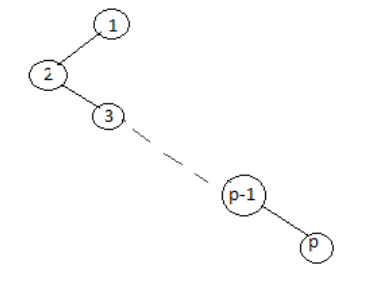
\includegraphics[width=45mm]{graf.png}
\end{figure}

\subparagraph{b1)}
Fie $T_k = T \backslash \{i_1, ..., i_{k-1}\}, \forall 1 \leq k \leq p-1 \Rightarrow V'=\{k, k+1, ..., p-1, p\}$. Și cum există o muchie între oricare
două noduri consecutive, rezultă că $d_{T_k} = 1, \forall k \Rightarrow i_k$ va fi mereu frunză în $T_k$.

\subparagraph{b2)}
Cum $V'=\{k, k+1, ..., p-1, p\}$, nodurile mai mici decât $k$ fiind eliminate și o altă frunză este $p \Rightarrow i_k$ este frunză minimă în $T_k$.  

\subparagraph{b3)}
Conform algoritmului, $T$-ul este un graf care conține $p-1$ muchii $\Rightarrow T$-ul este arbore.
Dacă formăm emblema acestuia respectând definiția din enunț, vom obține vectorul $x$, unde $x \in \{1,2,...,p\}^{p-1}$ cu $x_1=2, x_2=3, ...,x_{p-1}=p$.  

\end{document}